\documentclass[12pt,dvipdfmx]{report}
\usepackage{comment}
\usepackage{./sty/eclepsf}
\usepackage{tascmac}
\usepackage{tabularx}
\usepackage{listliketab}
\usepackage[longnamesfirst,numbers]{natbib}
\usepackage[dvipdfmx]{graphics}
\usepackage[dvipdfmx]{graphicx}
\usepackage[dvipdfmx]{color}
\usepackage{subfigure}
\usepackage{alltt}
\usepackage{here}
\usepackage{afterpage}
\usepackage{graphicx}
\usepackage{here}
\usepackage{amsmath, amssymb}
\usepackage{type1cm}
\usepackage{yquant}
\usepackage{tikz}
\usetikzlibrary{quantikz}
\usepackage{./sty/ncodeline}
%\usepackage[dvipdfmx, colorlinks, breaklinks,%
\usepackage[dvipdfmx, breaklinks,bookmarks=true, bookmarksnumbered=true,bookmarkstype=toc, bookmarksopen=true,bookmarksopenlevel=3,pdftitle={RG}]{hyperref}
\usepackage{bookmark}
\usepackage{mathtools}
\usepackage{tikz}
\usetikzlibrary{automata, positioning, arrows}
\usepackage[T1]{fontenc}

\AtBeginDvi{\special{pdf:tounicode EUC-UCS2}}

\usepackage{fancyhdr}

\usepackage{./sty/doxygenorig}

\usepackage{indentfirst}
\usepackage{url}
\usepackage{listings,./sty/jlisting}
\usepackage{float}
\graphicspath{ {./images/} }

\def\lstlistingname{プログラム}

\lstset{%
 language={C++},
 %backgroundcolor={\color[gray]{.85}},%
 basicstyle={\small\ttfamily},%
 identifierstyle={\small},%
 commentstyle={\small\itshape},%
 keywordstyle={\small\bfseries},%
 ndkeywordstyle={\small\ttfamily},%
 stringstyle={\small\ttfamily},
 frame={tb},
 framesep=1zw,
 breaklines=true,
 numbers=left,%
 xrightmargin=0zw,%
 xleftmargin=1.5zw,%
 numberstyle={\scriptsize},%
 stepnumber=1,
 numbersep=1zw,%
 lineskip=-0.5ex%
}

\usepackage{amssymb}
%\usepackage{supertabular,multirow}

\usepackage{array}
\newcolumntype{M}[1]{>{\centering\arraybackslash}m{#1}}

% A4  size: 297mm*210mm %1pt = 0.35mm
\setlength{\topmargin}{-3.4mm} % 10pt 25.4mm - 3.4mm = 22mm
\setlength{\oddsidemargin}{-0.4mm} % 25.4mm - 0.4mm = 25mm
\setlength{\evensidemargin}{-0.4mm} % 25.4mm - 0.4mm = 25mm
\setlength{\textheight}{231mm} % 660pt % original is 225.75mm 645pt
\setlength{\textwidth}{160mm} % 457pt

\renewcommand{\topfraction}{.99}
\renewcommand{\textfraction}{.0}
\renewcommand{\floatpagefraction}{.99}
\renewcommand{\bibname}{Reference}
\DeclareMathOperator{\tr}{tr}

\pagestyle{fancy}
\lhead[]{}

% タイトル
\def\title{Link Management in Quantum Network}
% 英語タイトル
\def\etitle{Link Management in Quantum Network}
% 著者(日本語)
\def\author{Makoto Nakai}
% 著者(英語)
\def\eauthor{Makoto Nakai}
% 学部・研究科
\def\dept{Keio University Graduate School of Media and Governance}
% 学部・研究科(英語)
\def\edept{Keio University Graduate School of Media and Governance}

\begin{document}

\pagenumbering{roman}
\begin{titlepage}
  \begin{spacing}{1.6}
  \begin{center}
  \Large 
   \textbf{Master's Thesis (Academic Year 2023)}\\
   \hspace*{\fill}\\
   \hspace*{\fill}\\
   \hspace*{\fill}\\
   \LARGE 
   \textbf{Link Management in a Quantum Network}
   \vspace{8.5cm}
   \end{center}
   \begin{flushleft}
       \Large 
       \textbf{Keio University \\ Graduate School of Media and Governance}
   \end{flushleft}
   \begin{flushright}
    \Large  
    \textbf{Makoto Nakai} 
   \end{flushright}
  \end{spacing}
\end{titlepage}

\thispagestyle{empty}

Abstract of master's Thesis - Academic Year 20xx
\begin{center}
\begin{large}
\begin{tabular}{|p{0.97\linewidth}|}
    \hline
      \etitle \\
    \hline
\end{tabular}
\end{large}
\end{center}

~ \\
 Quantum networking is the new paradigm of networking that allows to transfer quantum state and achieve various new applications.  RuleSet-based communication protocol is known to be one of the practical communication protocols to establish a scalable quantum network.
 Ideally, multiplexing and real-time resource management should be realized in order to improve the performance and robustness of the network. However, the protocol to handle multiple connections and allocate of physical links has not been proposed.
 This thesis proposes the link management protocol for quantum network that involves negotiation to determine a set of RuleSets (which is called a link allocation policy) to execute and the timing of apply the new link allocation policy.
 It also discusses the implementation of communication setup and teardown based on the proposed protocol and validates the proposed approach by performing a set of network simulations.
~ \\
Keywords : \\
\underline{1. Quantum Networking},
\underline{2. RuleSet-Based Communication Protocol},
\underline{3. Networking Protocol},
\begin{flushright}
\edept \\
\eauthor
\end{flushright}

\thispagestyle{plain}
\clearpage

\tableofcontents\thispagestyle{plain} %目次
\clearpage
\listoffigures\thispagestyle{plain} %図目次
\clearpage
\listoftables\thispagestyle{plain} %表目次
\clearpage

\pagenumbering{arabic}
\chapter{Introduction}
\label{introduction}

\section{Background}
\label{introduction:background} 

The recent development of quantum technologies such as quantum computing, quantum networking and quantum sensing are expected to provide new capabilities. 
For example, quantum processors can theoretically simulate quantum systems whose size are intractable even for their classical equivalence.
The key to realize these new applications is quantum effect, such as superposition and entanglement, both of which cannot be observed in the classical world.

However, there are two major problems for transmitting quantum data to a distance location, which is required in certain situations such as distributed quantum computing.
One is "non-cloning theorem", which is the fact that quantum state cannot be copied. Unlike classical network, it is almost impossible to neither amplify a quantum state or send it forward because the quantum state will be heavily corrupted by the high probability of loss and high error rate.
The other problem is that it is so difficult to establish a bell pair between nodes separated by a long distance, again due to a photon will be spoiled by the physical noise and photon loss.

These two problems can be solved by using particular type of nodes called quantum repeaters. Quantum repeaters perform entanglement swapping and purification, each of which extends two neighboring bell pairs to a single longer bell pair, and improves the fidelity of the bell pair, respectively.
These operations end up with generating an end-to-end bell pair that can be used by quantum teleportation, which is the protocol to send an arbitrary quantum state to a distant location. 

Entanglement swapping and purification involve requires frequent message exchange with neighboring nodes in order to coordinate actions, such as entanglement swapping and purification, with neighboring nodes and those communication slow down the generation of an end-to-end bell pair.
However, a communication protocol called RuleSet-based communication protocol solves this problem by distribute an object called RuleSet, which a sequence of operations execute to each node. This feature reduces the amount of unnecessary communication and improves the scalability of the entire network.

\section{Research Contribution}
\label{introduction:research-contribution}

Multiple connections should be established simultaneously in order to enhance the overall performance and robustness of the entire network and the same thing can be applied to quantum network. 
However, the previous work only proposes the method to allocate required physical bell pairs and establish a single end-to-end bell pair, in other word, an single connection by consuming those physical resources.
This thesis proposes a protocol to realize three important tasks, which are the negotiation about what set of connections are going to be established, the one about when to switch from those in the previous round, and coordinated resource management between two nodes connected by each link.
It also discusses the updated procedure of establishing a new connection and tearing down one of the existing connections while several connections are being established by applying the proposed protocol.
The proposed approach in this thesis is validated by the simulation of RuleSet-based quantum networks under several circumstances.

\section{Thesis Structure}
\label{introduction:thesis-structure} 
% 本論文における以降の構成は次の通りである.

% ~\ref{background}章では,背景を述べる.
% ~\ref{issue}章では,本研究における問題の定義と,解決するための要件の整理を行う.
% ~\ref{proposed}章では,本研究の提案手法を述べる.
% ~\ref{implementation}章では,~\ref{proposed}章で述べたシステムの実装について述べる.
% ~\ref{evaluation}章では,\ref{issue}章で求められた課題に対しての評価を行い,考察する.
% ~\ref{conclusion}章では,本研究のまとめと今後の課題についてまとめる.


%%% Local Variables:
%%% mode: japanese-latex
%%% TeX-master: "../thesis"
%%% End:

\chapter{Background}
\label{background}

\section{Quantum Physics}

\subsection{Quantum Bit}
A classical bit has two different states, which are 0 and 1.   Instead, those of a quantum bit (or \textbf{qubit} in short) are $|0\rangle$ and $|1\rangle$, each of which can be described as a vector. For example  
 $$|0\rangle = \Big[
\begin{array}{c}
1 \\
0 \\
\end{array}
\Big]
$$

$$|1\rangle = \Big[
\begin{array}{c}
0 \\
1 \\
\end{array}
\Big]$$

The state of a single 	qubit $|\psi\rangle$ can be described as follows.
$$ |\psi\rangle = \alpha |0\rangle + \beta |1\rangle \,(\alpha, \beta \in \mathbb{C}, |\alpha|^2+|\beta|^2=1)$$.
 After the operation called measurement, the quantum state would be collapsed into either 0 or 1.  The measurement probability of 0 is $|\alpha|^2$ and that of 1 is $|\beta|^2$. In other words, a single qubit can take both states probabilistically at the same time.  For instance, a qubit can be 
 
 \begin{equation}
	|\psi\rangle = \frac{1}{\sqrt{2}}|0\rangle + \frac{1}{\sqrt{2}}|1\rangle \tag{1}
\end{equation}

 which can be 50\% 0 and 50\% 1.

\subsection{Bloch sphere}
Because $|\alpha|^2 + |\beta|^2 = 1$, the notation of a single qubit state can be represented like this.

\begin{equation}
|\psi\rangle = e^{i\gamma} (\cos{\frac{\theta}{2}} + e^{i\phi} \sin{\frac{\theta}{2}}) (\gamma, \phi, \theta \in \mathbb{R})
\end{equation}.

Because $e^{i\gamma}$ is just a global state, it can be ignored and the same state can be rewritten like this.

\begin{equation}
 |\psi\rangle =  \cos{\frac{\theta}{2}} + e^{i\phi} \sin{\frac{\theta}{2}} (\phi, \theta \in \mathbb{C})
\end{equation}

Because the equation above has two parameters,  any pure single qubit state can be considered as a point on the surface and its geometric representation is called \textbf{Bloch sphere}.

\begin{figure}[ht]
  \centering
  \tikz{
    \tikzstyle{st}=[lightgray, fill, fill opacity=0.2];
    \coordinate(o)at(0,0); 
    \draw(o)circle(2cm); 
    \draw[fill](o)circle(1.5pt);%origin
    \draw[st](o)--(56.7:0.4)arc(56.7:90.:0.4)--cycle;%theta angle
    \draw(0.18,0.6)node{$\theta$};
    \draw[st](o)--(-135.7:0.4)arc(-135.7:-33.2:0.4)--cycle;%varphi angle
    \draw(0.14,-0.58)node{$\varphi$};
    \draw[->](o)--(-0.81,-0.79) node[above left]{\ $x$};%x
    \draw[->](o)--(2,0)node[right]{$y$};%y
    \draw[->](o)--(0,2)node[below right]{$z$}node[above]{\ $\ket{0}$};%z |0>
    \draw[rotate around={0.:(0.,0.)},dashed](0,0)ellipse(2cm and 0.9cm);%ellipse
    \draw[thick,->](o)--(0.70,1.07)node[above]{\ $\ket{\psi}$};%state vector
    \draw[densely dotted,->](o)--(0,-2)node[below]{\ $\ket{1}$};%-z |1>
    \draw[dotted](o)--(0.7,-0.46)--(0.7,1);%triangle
  }
    
\newpage
\caption{Bloch Sphere}
\end{figure}

\subsection{Multi-Qubit State}
  The quantum state for multi-qubits is a \textbf{tensor product} of a state vector of each qubit.  The general notation of two qubit state is
  
\begin{flalign}
    |\psi\rangle & = (\alpha |0\rangle + \beta |1\rangle) \otimes  (\gamma |0\rangle + \delta |1\rangle) \\
    & = \alpha \gamma |00\rangle + \alpha \delta |01\rangle + \beta \gamma |10\rangle + \beta \delta |11\rangle \\ 
   & (\alpha, \beta, \gamma, \delta \in \mathbb{C}, |\alpha|^2+|\beta|^2+|\gamma|^2+|\delta|^2=1)
 \end{flalign}.
  
  For example, the state $|00\rangle$ is equal to 
  
\begin{equation}
  \Big[
\begin{array}{c}
1 \\
0 \\
\end{array}
\Big]
\otimes
 \Big[
\begin{array}{c}
1 \\
0 \\
\end{array}
\Big]
= \Big[
\begin{array}{c}
1 \\
0 \\
0 \\
0 \\
\end{array}
\Big]
\end{equation}.

 However, some quantum states such as
 
 \begin{equation}
 	|\psi\rangle = \frac{1}{\sqrt{2}}|00\rangle + \frac{1}{\sqrt{2}}|11\rangle
 \end{equation}
 
 cannot be decomposed into quantum state of each qubit.  These special quantum states are called \textbf{entangled} states.

 \subsection{Mixed State}
 \subsection{Fidelity}
 \subsection{Quantum State Tomography}

\section{Quantum Operations}
\subsection{I Gate}

I gate is equal to the 2x2 identity matrix, which is 

\begin{equation}
I = \begin{bmatrix}
1 & 0 \\
0 & 1 \\
\end{bmatrix}
\end{equation}.

For example,

\begin{equation}
 I|0\rangle = \begin{bmatrix}
1 & 0 \\
0 & 1 \\
\end{bmatrix} 
\left[
\begin{array}{c}
1 \\
0 \\
\end{array}
\right]
= \left[
\begin{array}{c}
1 \\
0 \\
\end{array}
\right]
= |0\rangle
\end{equation}

\begin{equation}
I|1\rangle = \begin{bmatrix}
1 & 0 \\
0 & 1 \\
\end{bmatrix} 
\left[
\begin{array}{c}
0 \\
1  \\
\end{array}
\right]
= \left[
\begin{array}{c}
0 \\
1 \\
\end{array}
\right]
= |1\rangle
\end{equation}.

\subsection{X Gate}
\subsubsection{X gate}

X gate flips the logical value of a qubit.

\begin{equation}
X = \begin{bmatrix}
0 & 1 \\
1 & 0 \\
\end{bmatrix}
\end{equation}.

For example,
\begin{equation}
X|0\rangle = \begin{bmatrix}
0 & 1 \\
1 & 0 \\
\end{bmatrix} 
\left[
\begin{array}{c}
1 \\
0 \\
\end{array}
\right]
= \left[
\begin{array}{c}
0 \\
1 \\
\end{array}
\right]
= |1\rangle
\end{equation}

\begin{equation}
 X|1\rangle = \begin{bmatrix}
0 & 1 \\
1 & 0 \\
\end{bmatrix} 
\left[
\begin{array}{c}
0 \\
1  \\
\end{array}
\right]
= \left[
\begin{array}{c}
1 \\
0 \\
\end{array}
\right]
= |0\rangle
\end{equation}.

\subsection{Y Gate}

Y gate flips the logical value of a qubit and add an imaginary number.

\begin{equation}
 Y = \begin{bmatrix}
0 & -i \\
i & 0 \\
\end{bmatrix}
\end{equation}.

For example,
\begin{equation}
Y|0\rangle = \begin{bmatrix}
0 & -i \\
i & 0 \\
\end{bmatrix} 
\left[
\begin{array}{c}
1 \\
0 \\
\end{array}
\right]
= \left[
\begin{array}{c}
0 \\
i \\
\end{array}
\right]
= i|1\rangle
\end{equation}

\begin{equation}
Y|1\rangle = \begin{bmatrix}
0 & -i \\
i & 0 \\
\end{bmatrix} 
\left[
\begin{array}{c}
0 \\
1  \\
\end{array}
\right]
= \left[
\begin{array}{c}
-i \\
0 \\
\end{array}
\right]
= -i|0\rangle
\end{equation}.

\subsection{Z Gate}
Z gate flips the phase of $ |1\rangle$

\begin{equation}
 Z = \begin{bmatrix}
1 & 0 \\
0 & -1 \\
\end{bmatrix}
\end{equation}.

For example,
\begin{equation}
 Z|0\rangle = \begin{bmatrix}
1 & 0 \\
0 & -1 \\
\end{bmatrix} 
\left[
\begin{array}{c}
1 \\
0 \\
\end{array}
\right]
= \left[
\begin{array}{c}
1 \\
0 \\
\end{array}
\right]
= |0\rangle
\end{equation}

\begin{equation}
Z|1\rangle = \begin{bmatrix}
1 & 0 \\
0 & -1 \\
\end{bmatrix} 
\left[
\begin{array}{c}
0 \\
1  \\
\end{array}
\right]
= \left[
\begin{array}{c}
0 \\
-1 \\
\end{array}
\right]
= -|1\rangle
\end{equation}.

\subsection{H Gate}
H gate creates superposition.
\begin{equation}
 H = \frac{1}{\sqrt{2}}\begin{bmatrix}
1 & 1\\
1 & -1 \\
\end{bmatrix}
\end{equation}.

For example,
\begin{equation}
H|0\rangle = \frac{1}{\sqrt{2}}\begin{bmatrix}
1 & 1\\
1 & -1 \\
\end{bmatrix}\left[
\begin{array}{c}
1 \\
0 \\
\end{array}
\right]
= \frac{1}{\sqrt{2}} \left[
\begin{array}{c}
1 \\
1 \\
\end{array}
\right]
= \frac{1}{\sqrt{2}} (|0\rangle + |1\rangle)
\end{equation}

\begin{equation}
H|1\rangle = \begin{bmatrix}
1 & 1\\
1 & -1 \\
\end{bmatrix} 
\left[
\begin{array}{c}
0 \\
1  \\
\end{array}
\right]
= \frac{1}{\sqrt{2}} \left[
\begin{array}{c}
1 \\
-1 \\
\end{array}
\right]
=\frac{1}{\sqrt{2}} (|0\rangle - |1\rangle)
\end{equation}.

\subsection{Rotation Gate}
\subsection{General One Qubit Gate}

\subsection{Controlled-NOT Gate}
A CNOT gate involves two qubits, one is called \textbf{controlled qubit} and the other is called \textbf{target qubit}.  If the controlled qubit is 1, the bit value of the target qubit is flipped.

\begin{equation}
CNOT = \begin{bmatrix}
1 & 0 & 0 & 0 \\
0 & 1 & 0 & 0 \\
0 & 0 & 0 & 1 \\
0 & 0 & 1 & 0 \\
\end{bmatrix}
\end{equation}.

For example,
\begin{equation}
CNOT_{0,1}|10\rangle = 
\begin{bmatrix}
1 & 0 & 0 & 0 \\
0 & 1 & 0 & 0 \\
0 & 0 & 0 & 1 \\
0 & 0 & 1 & 0 \\
\end{bmatrix}
 \left[
\begin{array}{c}
0 \\
0 \\
1 \\
0 \\
\end{array}
\right]
=  \left[
\begin{array}{c}
0 \\
0 \\
0 \\
1 \\
\end{array}
\right] 
= |11\rangle 
\end{equation}

\begin{equation}
CNOT_{0,1}|11\rangle = 
\begin{bmatrix}
1 & 0 & 0 & 0 \\
0 & 1 & 0 & 0 \\
0 & 0 & 0 & 1 \\
0 & 0 & 1 & 0 \\
\end{bmatrix}
 \left[
\begin{array}{c}
0 \\
0 \\
0 \\
1 \\
\end{array}
\right]
=  \left[
\begin{array}{c}
0 \\
0 \\
1 \\
0 \\
\end{array}
\right] 
= |10\rangle 
\end{equation}.

\subsection{Measurement}
Quantum measurement can be described by using a group of measurement operators $\{M_m\}$
($m$ is the measurement result that is expected to get).
 If the quantum state before measurement is $|\psi\rangle$, the measurement probability of value $m$ is 
 $$p(m) = \langle \psi|M^{\dagger}_m M_m|\psi\rangle$$

 The quantum state after the measurement is 
 $$\frac{M_m|\psi\rangle}{\sqrt{\langle \psi|M^{\dagger}_m M_m|\psi\rangle}}$$

The measurement operators satisfy the completeness equation
$$\sum_{m} M^{\dagger}_m M_m = I$$

Also, the sum of the measurement probability of each possible measurement outcome is equal to one.
$$\sum_{m} p(m) = \langle \psi|\sum_{m} M^{\dagger}_m M_m|\psi\rangle = 1$$

\section{Quantum Circuit}
Here is the example of a quantum circuit.

\begin{figure}[ht]
  \begin{center}
    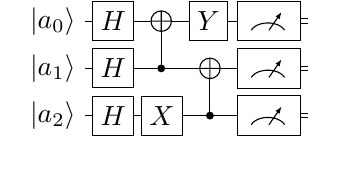
\begin{tikzpicture}
    \begin{yquant}
      qubit {$\ket{\reg_{\idx}}$} a[3];
      h a[0];
      h a[1];
      h a[2];
      cnot a[0] | a[1];
      x a[2];	
      y a[0];	 
      cnot a[1] | a[2]; 
      measure a[0-2];					 
     \end{yquant}
  \end{tikzpicture}
\caption{A example of quantum circuit}
\end{center}
\end{figure}

Each horizontal line represents each qubit and the square boxes that contain alphabets mean single quantum gates.  The sign which involves a vertical line means a CNOT gate, and the box on the most right side indicates measurement. 

\section{Quantum Entanglement}

Quantum entanglement is a special type of quantum state that cannot be described in the form of tensor product of the state of each particle.

\subsection{Bell Pair}
The entangled states between two qubits are called bell pairs, and each of four states has a special notation.
%% TODO: Add reference of EPR pair

\begin{equation}
  |\Phi^+\rangle = \frac{|00\rangle + |11\rangle}{\sqrt{2}}
  \end{equation}
  
  \begin{equation}
 |\Phi^-\rangle = \frac{|00\rangle - |11\rangle}{\sqrt{2}}
 \end{equation}
 
 \begin{equation}
 |\Psi^+\rangle = \frac{|01\rangle + |10\rangle}{\sqrt{2}}
 \end{equation}
 
 \begin{equation}
  |\Psi^-\rangle = \frac{|01\rangle - |10\rangle}{\sqrt{2}}
  \end{equation}.

\subsection{Multipartite Entanglement}
There are cases that more than two qubits are entangled and that state is called Greenberger–Horne–Zeilinger state or GHZ state.

Here is the braket notation of the GHZ state that involves three qubits.
\begin{equation}
  |GHZ\rangle = \frac{|000\rangle + |111\rangle}{\sqrt{2}}
\end{equation}.

In the general case, the braket notation of the GHZ state of N qubits is the following.
\begin{equation}
  |GHZ\rangle = \frac{|0\rangle^{\otimes N} + |1\rangle^{\otimes N}}{\sqrt{2}}
\end{equation}.

\subsection{Bell State Measurement}
Bell state measurement is a special type of quantum measurement that determines which bell pair the given two qubit entangled state is.
%% TODO: Add reference of BSM
\begin{figure}[ht]
  \begin{center}
    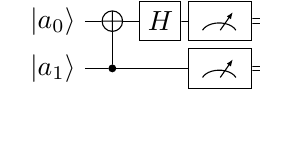
\begin{tikzpicture}
    \begin{yquant}
      qubit {$\ket{\reg_{\idx}}$} a[2];
      cnot a[0] | a[1];
      h a[0];	 
      measure a[0-1];					 
     \end{yquant}
  \end{tikzpicture}
\caption{Quantum circuit for bell state measurement}
\end{center}
\end{figure}

\begin{table}[ht]
  \begin{center}
    \begin{tabular}{|c|c|} \hline
      Measurement results & Bell state \\ \hline \cline{1-2}
      00 &  $|\Phi^+\rangle$ \\ \cline{1-2}
      01 & $|\Phi^-\rangle$ \\  \cline{1-2}
      10 &  $|\Psi^+\rangle$ \\ \cline{1-2}
      11 & $|\Psi^-\rangle$ \\  \hline  \cline{1-2}
    \end{tabular}
    \caption{A table of correspondence between measurement result and Bell pair}
  \end{center}
\end{table}

\subsection{Quantum Teleportation}

Unlike classical communication, quantum states cannot be just copied and transmit to other nodes due to the no-cloning theorem, which forbids duplication of any quantum state.  However, a method called quantum teleportation was proposed, which overcomes the restriction and allows sender to transmit single qubit state to a distant location. 
 		
This method requires both the single qubit state and a new Bell pair, and also the sender have to prepare two qubits and the receiver have to prepare one qubit.  After applying a CNOT gate and an H gate in the figure above, the sender have to measure both qubits and send those measurement results over the classical network.  After the receiver get those measurement results and apply some quantum gates if the measurement results of corresponding qubits on the sender's side are 1, in order to correct on the quantum state on the receiver's side.
%% TODO: Add reference of quantum teleportation (both idea and circuit)
%% TODO: Show that it works in the form of equations
%% TODO: Add reference of experimental works

\begin{figure}[ht]
  	\begin{center}
  		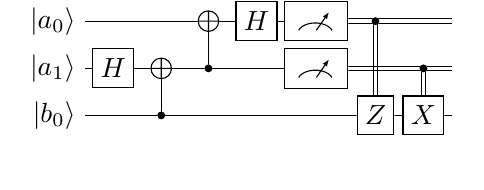
\begin{tikzpicture}
			\begin{yquant}
	 			qubit {$\ket{\reg_{\idx}}$} a[2];
	 			qubit {$\ket{\reg_{\idx}}$} b[1];
	 			h a[1];
        cnot a[1] | b[0];
	 			cnot a[0] | a[1];
        h a[0];	 
        measure a[0-1];	
        z b[0] | a[0];	
        x b[0] | a[1];				 
 			\end{yquant}
		\end{tikzpicture}
	\caption{Quantum circuit for quantum teleportation}
	\end{center}
\end{figure}

\newpage

\subsection{Entanglement Swapping}

Entanglement swapping is the method to extend quantum entanglement by performing joint measurement on several quantum entanglement.
For example, assume Alice has a single qubit, Bob has two qubits, and Charlie has one qubit. Then, there are Bell pairs between Alice's qubit and Bob's first qubit, and Bob's second qubit and Charlie's qubit, respectively.
If Bob performs Bell state measurement on both of his qubits, Alice's qubit and Charlie's qubit are eventually entangled, even though they have not interacted with each other.
This can be also seen as the teleporatation of a Bell pair by sending one of its particles.
Here is the figure of quantum circuit to perform entanglement swapping.
%% TODO: Add reference of entanglement swapping (both idea and circuit)
%% TODO: Show that it works in the form of equations
%% TODO: Add reference of experimental works

\begin{figure}[ht]
  \begin{center}
    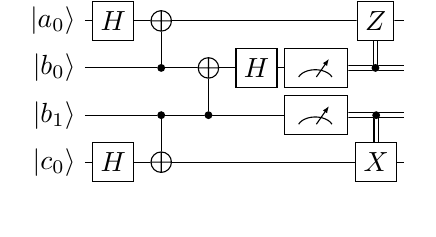
\begin{tikzpicture}
    \begin{yquant}
       qubit {$\ket{\reg_{\idx}}$} a[1];
       qubit {$\ket{\reg_{\idx}}$} b[2];
      qubit {$\ket{\reg_{\idx}}$} c[1];
       h a[0];
      h c[0];
       cnot a[0] | b[0];
       cnot c[0] | b[1];
      cnot b[0] | b[1];
      h b[0];	 
      measure b[0-1];	
      z a[0] | b[0];	
      x c[0] | b[1];		 
     \end{yquant}
  \end{tikzpicture}
\caption{Quantum circuit for entanglement swapping}
\end{center}
\end{figure}

\subsection{Entanglement Purification}
%% TODO: Add reference of entanglement purification (both idea and circuit)
%% TODO: Show that it works in the form of equations
%% TODO: Add reference of experimental works

Entanglement purification is a scheme to generate a set of quantum entanglements with higher fidelities from a larger set of imperfect quantum entanglements, local quantum operations, and classical communications.
This procedure is also called entanglement distillation, or quantum concatenation. This section presents an example of entanglement purification that generates a single bell pair with higher fidelity from two of those with less fidelity.

Assume Alice and Bob are supposed to share $|\Phi^+\rangle$, which is one of the Bell pairs. However, the state would be converted to the following mixed state due to the noisy nature of a quantum channel.
$$ \rho_{AB} = P_{\Phi^+}|\Phi^+\rangle\langle\Phi^+| + P_{\Phi^-}|\Phi^-\rangle\langle\Phi^-| + P_{\Psi^+}|\Psi^+\rangle\langle\Psi^+| + P_{\Psi^-}|\Psi^-\rangle\langle\Psi^-|$$

$$\sum_{s \in \{\Phi^+, \Phi^-, \Psi^+, \Psi^- \}} P_{s} = 1$$

Any mixed state can be converted to Werner state by applying Pauli operations and $\frac{\pi}{2}$ operations, so Alice and Bob can obtain the following state.

$$ \rho^{'}_{AB} = F|\Phi^+\rangle\langle\Phi^+| + \frac{1-F}{3}(|\Phi^-\rangle\langle\Phi^-| + |\Psi^+\rangle\langle\Psi^+| + |\Psi^-\rangle\langle\Psi^-|)$$

\begin{table}[ht]
  \begin{center}
    \begin{tabular}{|c|c|} \hline
      Before applying a CNOT gate & After a applying CNOT gate \\ \hline \cline{1-2}
      $|\Phi^+\rangle|\Phi^+\rangle$ &  $|\Phi^+\rangle|\Phi^+\rangle$ \\ \cline{1-2}
      $|\Phi^+\rangle|\Phi^-\rangle$ &  $|\Phi^-\rangle|\Phi^-\rangle$ \\ \cline{1-2}
      $|\Phi^+\rangle|\Psi^+\rangle$ &  $|\Phi^+\rangle|\Psi^+\rangle$ \\ \cline{1-2}
      $|\Phi^+\rangle|\Psi^-\rangle$ &  $|\Phi^-\rangle|\Psi^-\rangle$ \\ \cline{1-2}
      $|\Phi^-\rangle|\Phi^+\rangle$ &  $|\Phi^-\rangle|\Phi^+\rangle$ \\ \cline{1-2}
      $|\Phi^-\rangle|\Psi^-\rangle$ &  $|\Phi^+\rangle|\Phi^-\rangle$ \\ \cline{1-2}
      $|\Phi^-\rangle|\Psi^+\rangle$ &  $|\Phi^-\rangle|\Psi^+\rangle$ \\ \cline{1-2}
      $|\Phi^-\rangle|\Psi^-\rangle$ &  $|\Phi^+\rangle|\Psi^-\rangle$ \\ \cline{1-2}
      $|\Psi^+\rangle|\Phi^+\rangle$ &  $|\Psi^+\rangle|\Psi^+\rangle$ \\ \cline{1-2}
      $|\Psi^+\rangle|\Phi^-\rangle$ &  $|\Psi^+\rangle|\Psi^-\rangle$ \\ \cline{1-2}
      $|\Psi^+\rangle|\Psi^+\rangle$ &  $|\Psi^+\rangle|\Phi^+\rangle$ \\ \cline{1-2}
      $|\Psi^+\rangle|\Psi^-\rangle$ &  $|\Psi^+\rangle|\Phi^-\rangle$ \\ \cline{1-2}
      $|\Psi^-\rangle|\Phi^+\rangle$ &  $|\Psi^-\rangle|\Psi^+\rangle$ \\ \cline{1-2}
      $|\Psi^-\rangle|\Phi^-\rangle$ &  $|\Psi^-\rangle|\Psi^-\rangle$ \\ \cline{1-2}
      $|\Psi^-\rangle|\Psi^+\rangle$ &  $|\Psi^-\rangle|\Phi^+\rangle$ \\ \cline{1-2}
      $|\Psi^-\rangle|\Psi^-\rangle$ &  $|\Psi^-\rangle|\Phi^-\rangle$ \\ \cline{1-2}
    \end{tabular}
    \caption{A table of correspondence between Bell pairs before and after applying a CNOT gate}
  \end{center}
\end{table}

Two noisy bell pairs are required for entanglement purification, so assume the quantum state of the entire system can be described as follows.
\begin{multline*}
\rho^{'}_{a_1 b_1} \otimes \rho^{'}_{a_2 b_2} = F^2|\Phi^+\rangle|\Phi^+\rangle\langle\Phi^+|\langle\Phi^+| \\ 
+ \frac{F(1-F)}{3}(|\Phi^+\rangle|\Phi^-\rangle\langle\Phi^-|\langle\Phi^+|+|\Phi^+\rangle|\Psi^+\rangle\langle\Psi^+|\langle\Phi^+|+|\Phi^+\rangle|\Psi^-\rangle\langle\Psi^-|\langle\Phi^+| \\
+|\Phi^-\rangle|\Phi^+\rangle\langle\Phi^+|\langle\Phi^-|+|\Psi^+\rangle|\Phi^+\rangle\langle\Phi^+|\langle\Psi^+|+|\Psi^-\rangle|\Phi^+\rangle\langle\Phi^+|\langle\Psi^-|) \\ 
+ \frac{(1-F)^2}{9}(|\Phi^-\rangle|\Phi^-\rangle\langle\Phi^-|\langle\Phi^-|+|\Phi^-\rangle|\Psi^+\rangle\langle\Psi^+|\langle\Phi^-|+|\Phi^-\rangle|\Psi^-\rangle\langle\Psi^-|\langle\Phi^-| \\
+ |\Psi^+\rangle|\Phi^-\rangle\langle\Phi^-|\langle\Psi^+|+|\Psi^+\rangle|\Psi^+\rangle\langle\Psi^+|\langle\Psi^+|+|\Psi^+\rangle|\Psi^-\rangle\langle\Psi^-|\langle\Psi^+| \\
+|\Psi^-\rangle|\Phi^-\rangle\langle\Psi^-|\langle\Phi^-|+|\Psi^-\rangle|\Psi^+\rangle\langle\Psi^+|\langle\Psi^-|+|\Psi^-\rangle|\Psi^-\rangle\langle\Psi^-|\langle\Psi^-|)
\end{multline*}

One of the bell pair $\rho^{'}_{a_1 b_1}$ is called source bell pair, which may be purified, and the other one $\rho^{'}_{a_2 b_2}$  is called target bell pair, which is going to be measured. Then, Alice and Bob perform CNOT operations between $a_1$ and $a_2$, and $b_1$ and $b_2$, respectively.
The entire quantum state on this point would be as follows.
\begin{multline*}
  \rho^{'}_{a_1 b_1} \otimes \rho^{'}_{a_2 b_2} = F^2|\Phi^+\rangle|\Phi^+\rangle\langle\Phi^+|\langle\Phi^+| \\ 
  + \frac{F(1-F)}{3}(|\Phi^-\rangle|\Phi^-\rangle\langle\Phi^-|\langle\Phi^-|+|\Phi^+\rangle|\Psi^+\rangle\langle\Psi^+|\langle\Phi^+|+|\Phi^-\rangle|\Psi^-\rangle\langle\Psi^-|\langle\Phi^-| \\
  +|\Phi^-\rangle|\Phi^+\rangle\langle\Phi^+|\langle\Phi^-|+|\Psi^+\rangle|\Psi^+\rangle\langle\Psi^+|\langle\Psi^+|+|\Psi^-\rangle|\Psi^+\rangle\langle\Psi^+|\langle\Psi^-|) \\ 
  + \frac{(1-F)^2}{9}(|\Phi^+\rangle|\Phi^-\rangle\langle\Phi^-|\langle\Phi^+|+|\Phi^-\rangle|\Psi^+\rangle\langle\Psi^+|\langle\Phi^-|+|\Phi^+\rangle|\Psi^-\rangle\langle\Psi^-|\langle\Phi^+| \\
  + |\Psi^+\rangle|\Psi^-\rangle\langle\Psi^-|\langle\Psi^+|+|\Psi^-\rangle|\Phi^+\rangle\langle\Phi^+|\langle\Psi^+|+|\Psi^+\rangle|\Psi^-\rangle\langle\Psi^-|\langle\Psi^+| \\
  +|\Psi^-\rangle|\Psi^-\rangle\langle\Psi^-|\langle\Psi^-|+|\Psi^-\rangle|\Phi^+\rangle\langle\Phi^+|\langle\Psi^-|+|\Psi^-\rangle|\Phi^-\rangle\langle\Phi^-|\langle\Psi^-|)
  \end{multline*}

After that, they measure $a_2$ and $b_2$ respectively, which is the qubit on the target bell pair on their side and exchange the measurement results.  

If their measurement results match, the purification is successful, while they have to discard the source bell pair and try again if those results do not match.

Here is the quantum state after measuring the target bell pair.

\begin{multline*}
\rho^{'}_{ab} = \frac{1}{N} \big[ F^2 + \frac{1}{9}\big(1-F \big)^2\big]|\Phi^+\rangle\langle\Phi^+| + \frac{2F(1-F)}{3N}|\Phi^-\rangle\langle\Phi^-| + \frac{2(1-F)^2}{9N}(|\Psi^+\rangle\langle\Psi^+| + |\Psi^-\rangle\langle\Psi^-|) \\
(N = F^2 + \frac{2F(1-F)}{3} + \frac{2(1-F)^2}{9})
\end{multline*}

The purification becomes successful if F  $> \frac{1}{2}$

\section{Quantum Networking}
\subsection{Quantum Node}
\subsection{Quantum Repeater}
\subsection{Quantum Link}
\subsection{Major Applications of Quantum Networking}


\chapter{Related Works}
\label{related works}

\section{Link Layer Protocol For Quantum Network}

\section{RuleSet-Based Quantum Network}

\chapter{Problem Definition}
\label{problem-definition}

\section{Problem Definition}

In order to maximize the overall performance and the aggregative use of resources in the entire network, it is desirable for several connections to be established in the real-time fashion.
However, there are two major obstacles to overcome in the case of a quantum network. 

One is the absence of a link management protocol for quantum network. There is previous work \cite{aparicio2011multiplexing} that proposes and compares the performance of various multiplexing strategies, but it does not mention any concrete methods to establish multiple connections and allocate the available physical links to each of these connections.

The other one is the lack of interaction between connection management and the subsequent resource management. The current RuleSet-based communication protocol \cite{matsuo2019quantum} only proposes the scheme to establish a single connection and it does not explain the method to tear it down and free the allocated physical links after the end of RuleSet execution. 

This thesis tackles the first problem by proposing the link management protocol the involves the negotiation about the set of connections to establish and the one about when to start the establishment. It also discuss the messages and their properties that are required to run this protocol.

Additionally, this thesis explains how the link management scheme is going to be triggered when a new connection is established and the old one is torn down. This explanation includes the methods to implement in the relevant software components when RuleSet-based quantum network is simulated or deployed in the real world.

\section{Assumptions}

This protocol is proposed based on the following assumptions.

\begin{itemize}
  \item The behavior of the entire network is determined by the collective decision made by each node.
  \item Each node allows the increase or decrease of the number of ongoing connections and does not refuse the setup of the new connection.
  \item The Bell pairs that are allocated but not used will be reallocated to one of the new connections.
  \item The link management protocol is triggered by the notification of either the setup of a new connection, or the teardown of an existing connection.
  \item The same amount of Bell pairs will be allocated to each RuleSet.
\end{itemize}

\section{Requirements}

This protocol has several requirements as follows.

\subsection{Functional requirements}

\subsubsection{Common}

\begin{itemize}
  \item Two neighboring nodes MUST agree on the next set of RuleSets (which is called the link allocation policy) and its order.
\end{itemize}

\subsubsection{Connection Setup}

\begin{itemize}
  \item Two neighboring nodes MUST also agree with when the new policy will be applied.
  \item If these negotiations are successful, available Bell pairs on the link level MUST be allocated to one of the RuleSets in the next link allocation policy.
\end{itemize}

\subsubsection{Connection Teardown}
\begin{itemize}
\item The execution of the old RuleSet MUST be terminated.
\item Link Bell pairs that are allocated but not consumed MUST be released from the RuleSet after its connection is terminated.
\end{itemize}


%%% Local Variables:
%%% mode: japanese-latex
%%% TeX-master: "./thesis"
%%% End:

\chapter{Proposal}
\label{proposal}

hoge

\section{hoge}



%%% Local Variables:
%%% mode: japanese-latex
%%% TeX-master: "../bthesis"
%%% End:

\chapter{Simulation}
\label{simulation}

\section{QuISP (Quantum Internet Simulation Package)}

\subsection{Overview}

QuISP \cite{satoh2022quisp} is a quantum network simulator which aims to simulate the behavior of a large-scale quantum network. It is built on top of OMNeT++ \cite{10.5555/1416222.1416290}, which is an event-driven network simulator.
The reason why QuISP is built on top of OMNet++ is that OMNet++ allows users to define their own networking layers.
QuISP can simulate various types of errors, not only Pauli X error, Pauli Y error and Pauli Z error, but also relaxation error and excitation error.
Physical noise on an actual quantum system with $n$ qubits are usually simulated in the form of a density matrix, which would includes $2^n \times 2^n$ elementss and soon becomes intractable as $n$ becomes larger.
QuISP realizes the scalable simulation of quantum network by simulating the physical error using an error probability vector, which would take the following form.

\begin{equation}
  \overrightarrow{\pi}(t) = (\pi_I, \pi_X, \pi_Y, \pi_Z, \pi_R, \pi_E, \pi_L)
\end{equation}
It contains $m+1$ elements (m is the number of simulated error types)
The time evolution of error probability vector is provided by a transition error matrix $Q$.
\begin{equation}
  \overrightarrow{\pi}(t) = \overrightarrow{\pi}(t-1)Q 
\end{equation}

The error probability vector above is the one for a single qubit, so the one for $N$ qubit system contains $N(m+1)$ elements.

\subsection{Hardware Components}

Communication between two quantum nodes is achieved by transmission of photons via an optical fiber, and the fiber is mocked by an object called quantum link.
QuISP supports three main link architecture. 

\subsubsection{Memory-Memory}
The first one is Memory-Memory that two nodes are directly connected via a quantum link and the Bell State Analyzer is equipped in the receiver node.

\subsubsection{Memory-Interface-Memory}
The second one is Memory-Interface-Memory. Both end nodes of a quantum link emits photons to Bell State Analyzer located in the middle. After they become entangled, all the measurements results and required operations are sent back to both nodes.

\subsubsection{Memory-Source-Memory}
The last one Memory-Source-Memory. All the entanglement pairs are both generated and sent from the source of entangled photonic pair states in the middle.

\subsection{Software Components}

\subsubsection{Connection Manager}

Connection establishment is done when connection manager at the Initiator nodes sends ConnectionSetupRequest to the Responder node and intermediate nodes sends additional information such as those about QNIC.
After that, the connection manager at the responder node sends ConnectionSetupResponse to each node along the path of the connection.

\subsubsection{Hardware Monitor}
Hardware monitor is the module that collects the information of a quantum link such as fidelity and generation rate and pass those information to the routing daemon and the connection manager.

\subsubsection{Bell Pair Store}
Bell pair store is the module that stores the entanglement pairs generated from a support node such as a Bell State Analyzer.

\subsubsection{Rule Engine}
Rule engine is the component that is in charge for executing the given RuleSets and monitor the conditions of physical qubits.

\subsubsection{Real-Time Controller}
Real-time controller is the component that is responsible for the initialization of physical components and coordination of the timing for photon emission.

\subsubsection{Routing Daemon}
Routing daemon is the component that generates and exchanges the routing table for quantum network interface card, or QNIC in short.

\section{Implementation}

This section discusses the mechanism and required methods that the author implemented in order to realize link management in QuISP.

\subsection{Physical Resource Management}

\subsection{Link Management}
\subsubsection{Link Allocation Policy Negotiation}
\subsubsection{Link Allocation Timing Negotiation}
\subsubsection{Resource Allocation}

\subsection{Connection Management}


%%% Local Variables:
%%% mode: japanese-latex
%%% TeX-master: "../bthesis"
%%% End:

\chapter{Evaluation}
\label{evaluation}

\section{Experiment}

The author performed several experiments using QuISP (Quantum Internet Simulation Package) and demonstration of the proposed protocol in several circumstances.

\subsection{Two Node Network With an MM Link}
Both nodes coordinated both the upcoming link allocation policy and the sequence number of the first available physical entanglement pair.

\subsection{Two Node Network With an MIM Link}
Both nodes coordinated both the upcoming link allocation policy and the sequence number of the first available physical entanglement pair.

% \subsection{Two Node Network With an MSM Link}
% \subsection{Two Node Network With an MIM Link (Without Timing Negotiation)}



%%% Local Variables:
%%% mode: japanese-latex
%%% TeX-master: "./thesis"
%%% End:

\chapter{Conclusion}
\label{conclusion}

\section{Conclusion}

This thesis proposed the link management protocol for quantum network, which provides coordinated decision about two aspects.
One is the upcoming link allocation policy, which are the list of RuleSets, or operations each node needs to execute in order to establish an end-to-end connection.
The other one is the particular Bell pair that the next link allocation policy should be applied to.
Also, the author validated the approach by performing several simulation for a RuleSet-based quantum network.

\section{Future work}

The quantum network requires more advanced multiplexing methods, such as a prioritized multiplexing, in order to enhance the overall performance of the entire network.
It is also desirable to develop congestion control techniques for a quantum network to figure out the better use of resources and void congestion control on the overall network.

%%% Local Variables:
%%% mode: japanese-latex
%%% TeX-master: "../thesis"
%%% End:

\appendix
\chapter{Appendix}


\section{hoge}



\chapter*{Acknowledgement}
\addcontentsline{toc}{chapter}{Acknowledgement}
\label{acknowledgement}

First and formost, I would like to express my deepest gratitude to Professor Rodney Van Meter, who has supervised my research activities in the last six years in AQUA.
Also, I would like to thank Dr.Takahiko Satoh, who is now an associate professor at the School of Science and Engineering, for his patient to nurture my ability to come up with all the aspects of my research, such as problem definition, proposal, implementation and presentation.
Additionally, I would like to thank Dr






%%% Local Variables:
%%% mode: japanese-latex
%%% TeX-master: "../yummy_bthesis"
%%% End:


% \renewcommand{\thechapter}{\Alph{chapter}}
% \setcounter{chapter}{0}
% \vspace{-5mm}


\input{bib/biblio}\thispagestyle{plain}%bibtex

\end{document}

%%% Local Variables:
%%% mode: japanese-latex
%%% TeX-master: t
%%% End:
